\subsection{Struktura}\label{subsec:struktura}
W sumie przeanalizowanych zostało 135 zestawów danych.
Pojedynczy zestaw danych składa się z pomiarów czujników rozmieszczonych w różnych miejscach na pojedynczym obiekcie.
Liczba czujników waha się od kilku do kilkudziesięciu.
Każdy czujnik jest scharakteryzowany przez następujące dane:
\begin{itemize}
    \item identyfikator,
    \item odległość bazowa — oznaczająca odległość zmierzoną przez laserowe urządzenie pomiarowe, w chwili uruchomienia monitoringu na obiekcie,
    \item seria pomiarów — notująca odległość czujnika od podłoża w kolejnych momentach.
\end{itemize}
Rozwiązanie zostało opracowane na podstawie pomiarów 1225 urządzeń i około 600 tys.\ pomiarów odległości.

\subsection{Charakterystyka}\label{subsec:charakterystyka}

\subsubsection{Odstępy czasu}
\begin{figure}[h]
    \centering
    % This file was created with tikzplotlib v0.9.12.
\begin{tikzpicture}

\definecolor{color0}{rgb}{0.886274509803922,0.290196078431373,0.2}

\begin{axis}[
axis background/.style={fill=white!89.8039215686275!black},
axis line style={white},
log basis y={10},
tick align=outside,
tick pos=left,
x grid style={white},
xlabel={Odstępy czasu między kolejnymi pomiarami [minuty]},
xmajorgrids,
xmin=98.5, xmax=1341.5,
xtick style={color=white!33.3333333333333!black},
y grid style={white},
ylabel={liczba wystąpień},
ymajorgrids,
ymin=119.838906477549, ymax=6012830.80078,
ymode=log,
ytick style={color=white!33.3333333333333!black}
]
\draw[draw=black,fill=color0,line width=0.48pt] (axis cs:335,0) rectangle (axis cs:385,1873303);
\draw[draw=black,fill=color0,line width=0.48pt] (axis cs:155,0) rectangle (axis cs:205,3676383);
\draw[draw=black,fill=color0,line width=0.48pt] (axis cs:695,0) rectangle (axis cs:745,1595);
\draw[draw=black,fill=color0,line width=0.48pt] (axis cs:515,0) rectangle (axis cs:565,611);
\draw[draw=black,fill=color0,line width=0.48pt] (axis cs:1055,0) rectangle (axis cs:1105,479);
\draw[draw=black,fill=color0,line width=0.48pt] (axis cs:1235,0) rectangle (axis cs:1285,196);
\draw[draw=black,fill=color0,line width=0.48pt] (axis cs:875,0) rectangle (axis cs:925,235);
\end{axis}

\end{tikzpicture}

    \captionof{figure}{Zbiorczy histogram przedstawiający odstępy czasu między kolejnymi pomiarami dla wszystkich danych.}\label{fig:odstepyczasu}
\end{figure}

Rysunek~\ref{fig:odstepyczasu} pokazuje, że przez większość czasu okres raportowania wynosi 3 lub 6 godzin.
By ułatwić komputerową analizę, dane zostały przepróbkowane do jednostajnego okresu 3h.
Finalnie, każdy okres jest reprezentowany przez jedną wartość pomiaru.
Każdy przedział czasu z co najmniej jednym pomiarem jest zagregowany do mediany.
Każdy przedział 3-godzinny bez żadnego pomiaru jest reprezentowany przez ostatni pomiar przed tym przedziałem.

Mediana jest tutaj właściwym agregatorem, ponieważ jest ona odporna na duże odchylenia, w przeciwieństwie do np.\ średniej.

\subsubsection{Różnice odległości między kolejnymi pomiarami}

\begin{figure}[h]
    \centering
    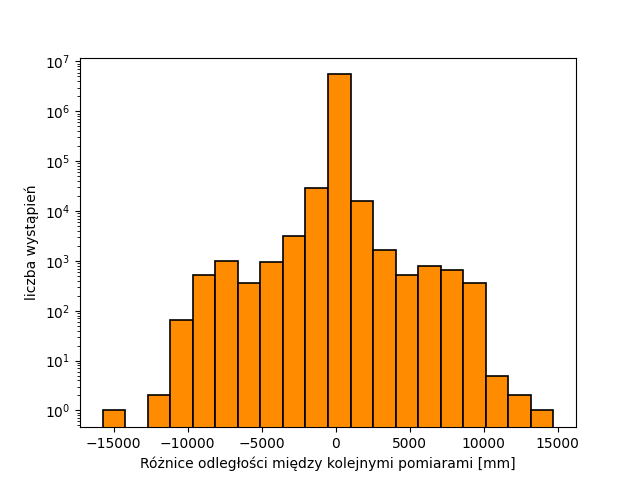
\includegraphics[width=\textwidth]{dist_diff_big.png}\captionof{figure}{Zbiorczy histogram różnic między kolejnymi pomiarami odległości dla wszystkich danych.}
    \label{fig:distbig}
\end{figure}

Bardzo istotne jest to, że na rysunku~\ref{fig:distbig} pionowa skala jest logarytmiczna.
Z informacji dostarczonych przez firmę wiadomo, że bez zastawienia czujnika, różnica pomiaru w ciągu kilku godzin może być co najwyżej 25-milimetrowa.
Ta informacja pokrywa się z wyżej pokazanym wykresem, ponieważ zdecydowana większość obserwacji jest zawarta w tym zakresie.
Bardzo wysoki szpic do 10 milimetrów reprezentuje zdecydowaną większość obserwacji, co widać na rysunku~\ref{fig:diffsmall}.


\begin{figure}[h]
    \centering
    % This file was created with tikzplotlib v0.9.12.
\begin{tikzpicture}

\definecolor{color0}{rgb}{0.886274509803922,0.290196078431373,0.2}

\begin{axis}[
axis background/.style={fill=white!89.8039215686275!black},
axis line style={white},
log basis y={10},
tick align=outside,
tick pos=left,
x grid style={white},
xlabel={Różnice odległości między kolejnymi pomiarami [mm]},
xmajorgrids,
xmin=-26.95, xmax=26.95,
xtick style={color=white!33.3333333333333!black},
y grid style={white},
ylabel={liczba wystąpień},
ymajorgrids,
ymin=226.106279176677, ymax=6677184.14321567,
ymode=log,
ytick style={color=white!33.3333333333333!black}
]
\draw[draw=black,fill=color0,line width=0.48pt] (axis cs:-24.5,0) rectangle (axis cs:-22.05,364);
\draw[draw=black,fill=color0,line width=0.48pt] (axis cs:-22.05,0) rectangle (axis cs:-19.6,646);
\draw[draw=black,fill=color0,line width=0.48pt] (axis cs:-19.6,0) rectangle (axis cs:-17.15,548);
\draw[draw=black,fill=color0,line width=0.48pt] (axis cs:-17.15,0) rectangle (axis cs:-14.7,868);
\draw[draw=black,fill=color0,line width=0.48pt] (axis cs:-14.7,0) rectangle (axis cs:-12.25,803);
\draw[draw=black,fill=color0,line width=0.48pt] (axis cs:-12.25,0) rectangle (axis cs:-9.8,1615);
\draw[draw=black,fill=color0,line width=0.48pt] (axis cs:-9.8,0) rectangle (axis cs:-7.35,1816);
\draw[draw=black,fill=color0,line width=0.48pt] (axis cs:-7.35,0) rectangle (axis cs:-4.9,6412);
\draw[draw=black,fill=color0,line width=0.48pt] (axis cs:-4.9,0) rectangle (axis cs:-2.45,25374);
\draw[draw=black,fill=color0,line width=0.48pt] (axis cs:-2.45,0) rectangle (axis cs:0,1174980);
\draw[draw=black,fill=color0,line width=0.48pt] (axis cs:0,0) rectangle (axis cs:2.45,4182142);
\draw[draw=black,fill=color0,line width=0.48pt] (axis cs:2.45,0) rectangle (axis cs:4.9,20956);
\draw[draw=black,fill=color0,line width=0.48pt] (axis cs:4.9,0) rectangle (axis cs:7.35,5312);
\draw[draw=black,fill=color0,line width=0.48pt] (axis cs:7.35,0) rectangle (axis cs:9.8,1646);
\draw[draw=black,fill=color0,line width=0.48pt] (axis cs:9.8,0) rectangle (axis cs:12.25,1517);
\draw[draw=black,fill=color0,line width=0.48pt] (axis cs:12.25,0) rectangle (axis cs:14.7,760);
\draw[draw=black,fill=color0,line width=0.48pt] (axis cs:14.7,0) rectangle (axis cs:17.15,824);
\draw[draw=black,fill=color0,line width=0.48pt] (axis cs:17.15,0) rectangle (axis cs:19.6,468);
\draw[draw=black,fill=color0,line width=0.48pt] (axis cs:19.6,0) rectangle (axis cs:22.05,577);
\draw[draw=black,fill=color0,line width=0.48pt] (axis cs:22.05,0) rectangle (axis cs:24.5,361);
\end{axis}

\end{tikzpicture}

    \captionof{figure}{Zbiorczy histogram różnic między kolejnymi pomiarów odległości dla wszystkich danych. Obcięty do 25mm.}
    \label{fig:diffsmall}
\end{figure}

\subsubsection{Różnice bazy od odległości}
\begin{figure}[h]
    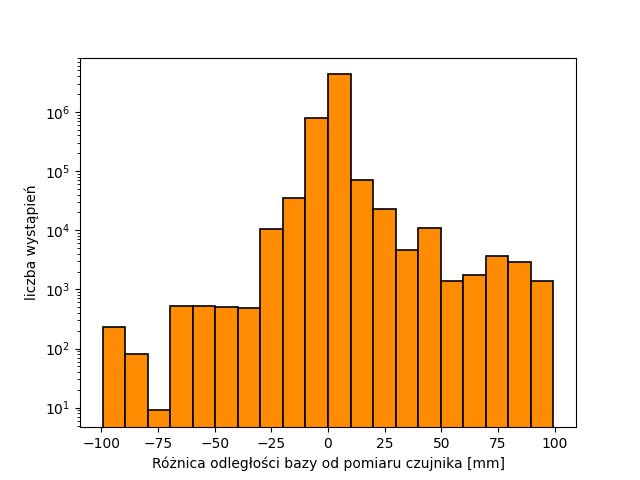
\includegraphics[width=\textwidth]{dist_histogram_100.png}
    \captionof{figure}{Zbiorczy histogram różnic odległości bazowej od pomiarów odległości.}
    \label{fig:dist}
\end{figure}


Dane na rysunku~\ref{fig:dist} są ponownie przedstawione w skali logarytmicznej, bo w przeciwnym wypadku nie dałoby się niczego zauważyć.
Zdecydowana większość obserwacji oscyluje wokół zera.
Mediana jest równa zero.
Będzie to kluczowe — prawdziwe ugięcia dachu powinny być krótkotrwałe i w dłuższej perspektywie mediana pomiarów powinna wynosić zero.

\subsubsection{Autokorelacja}\label{subsubsec:autocorrelation}

Na rysunku~\ref{fig:autocorrelation} pokazana jest zbiorcza autokorelacja wszystkich szeregów czasowych pomiarów z każdego czujnika, indeksowana przesunięciem (ang.\ lag).
Niebieskim cieniem jest zaznaczony przedział ufności (ang.\ \emph{confidence interval}), który pokazuje które korelacje są statystycznie istotne.

Zatem autokorelacja jest na tyle statystycznie istotna, że można zamodelować szereg czasowy pomiarów czujników autoregresją z oknem o długości 20.
\begin{figure}[H]
    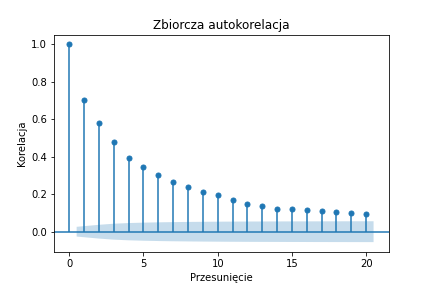
\includegraphics[width=0.9\textwidth]{autocorrelation.png}
    \captionof{figure}{Zbiorcza autokorelacja różnicy odległości bazowej od pomiaru dla wszystkich zestawów danych.}
    \label{fig:autocorrelation}
\end{figure}

\subsubsection{Omówienie wybranych przykładów}

Dane z urządzenia \hyperref[fig:example812]{JTI OTP - Gostków Stary/P-3}, pokazują przykład zastawienia 13mm trwającego przez wrzesień roku 2020.
Natomiast ostatnia część wykresu pokazuje faktyczne ugięcie dachu spowodowane śniegiem w lutym 2021.
Wspomniane warunki pogodowe wyróżniają się np.\ również w danych z urządzenia \hyperref[fig:example201]{C-Lublin - Lublin /P4}.


